\section{Koord Language and Semantics}
\label{sec:semantics}
The interaction model of an agent executing a $\lgname$ program is shown in \reffig{arch}. 
\begin{figure}[h!]
\centering
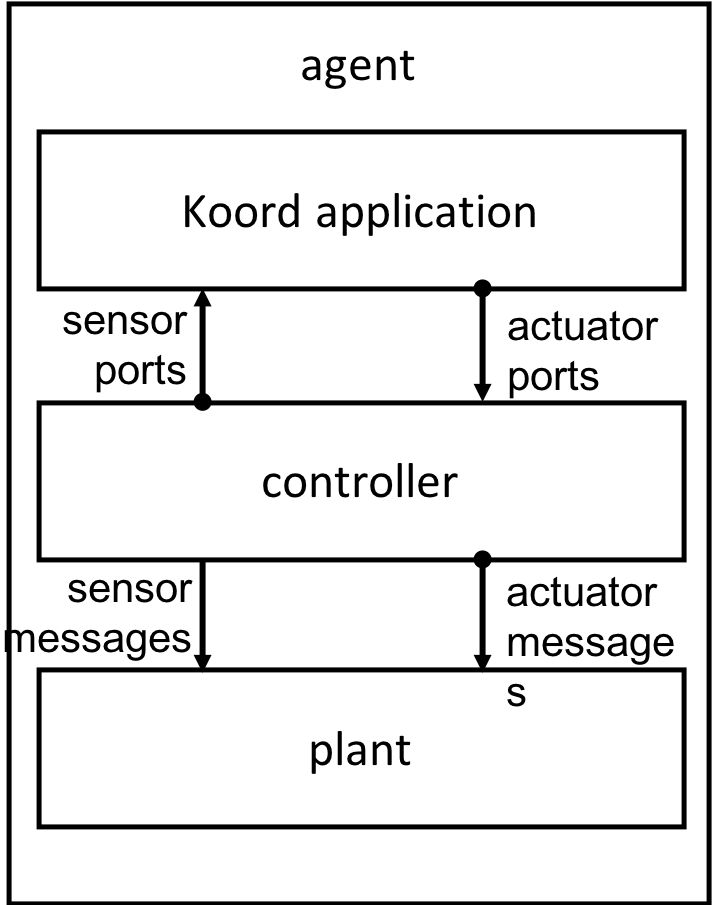
\includegraphics[width=0.23\textwidth]{figs/arch.png}
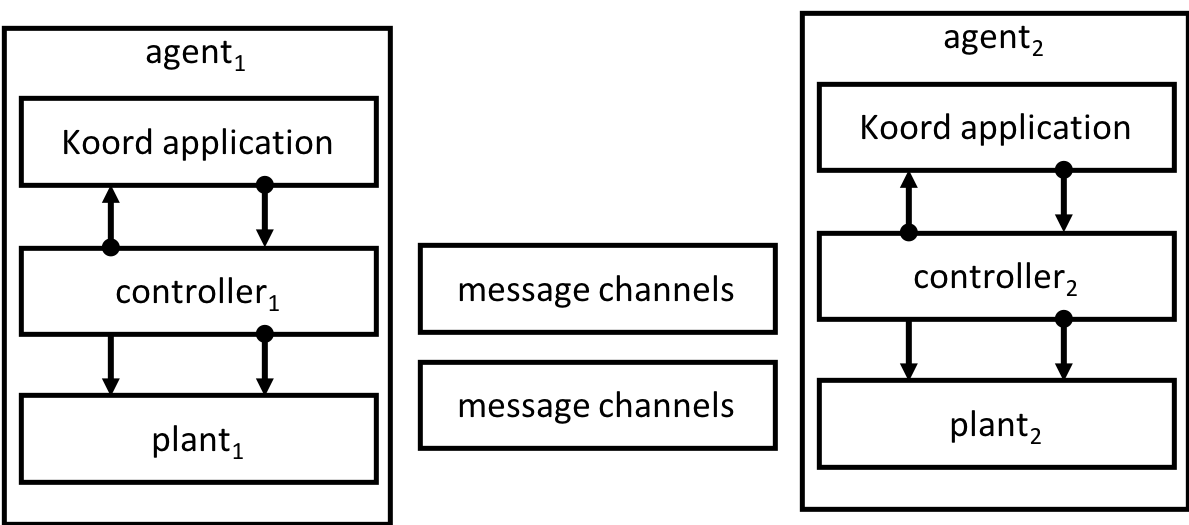
\includegraphics[width=0.24\textwidth]{figs/agents2.png}
\caption{\small An agent executing a $\lgname$ application and interacting with the physical environment through sensor and actuator ports ({\em left}). Interaction across multiple agents happens through shared variables implmented over message passing ({\em right}).}
\label{fig:arch}
\end{figure}
The program and the controller interact with each other through {\em sensor} and {\em actuator} ports.  The program reads the sensor ports, reads and writes to program variables, and writes to actuator ports. The controller drives the underlying physical plant. The \emph{environment} of a  $\lgname$ program is the combination of the controller and the plant. The set of agents in the system may interact with each other using {\em shared variables\/}. Each agent in the system runs an instance of the \emph{same} $\lgname$ program. 
% exmaple code snippet
\begin{figure}[ht!]
    \noindent
    \begin{mdframed}

    \begin{center}
        \scriptsize
        \two{0.4}{0.6}
        {\lstinputlisting[language=xyzNums,firstline=1,lastline=23,frame=none]{code/tasks_new.tex}}
        {\lstinputlisting[language=xyzNums,firstline=24,frame=none,firstnumber=24]{code/tasks_new.tex}}
    \end{center}
    \end{mdframed}

    \caption{$\lgname$ program for robot $i$ to do required tasks at provided locations.}
    \label{fig:taskapp}
\end{figure}
    
\paragraph* {A distributed $\mathit{Task}$ allocation application} \reffig{taskapp} shows a distributed task allocation application written in $\lgname$. This app involves mutual exclusion as well as construction of de-conflicted  paths. Tasks are abstractions for real location-based objectives like package delivery, surveillance, or fire-fighting.  Koord enables implementation of simple task allocation strategies using shared variables. In $\mathit{Task}$ app, the agents maintain a shared list of tasks ({\em taskList}) to complete, and each agent is uniquely assigned a task from this list in the event {\em Assign}. Once an agent reaches the task location (event {\em Reached}), it does whatever the task entails (event {\em Complete}), and continues this process.
% language features - what main "issue" each feature addresses . 

\subsection{Koord model for distributed CPS}
$\lgname$ design comprises of a \emph{turn}-based alternating semantics of discrete and dynamic behavior of each agent in the distributed system. The agents can be viewed as performing \emph{rounds} of execution, where each round consists of a \begin{inparaenum} 
\item \emph{a program transition} which is a discrete computational step, and 
\item \item \emph{an environment transition} which is the dynamic behavior of the controller, environment, and their effect on the sensors and actuators
\end{inparaenum}. 
In our semantics, we record whether it is the turn for a program transition or an environment transition  by a special $\mathit{turn}$ variable.  

In a program transition in a round, each agent first nondeterministically chooses an \emph{enabled} event, or an event whose precondition evaluates to \verb|True|. It then executes the statements in the effect of that event. %This may involve reading sensor ports, performing computations using local and shared variables, and writing to actuator ports. 
Then, the agent performs the environment transition in the round, during which it interacts with the physical environment and behaves as dictated by the actuator ports on the controller for $\delta$ amount of time.  \footnote{ $\delta>0$ is a constant \emph{sampling period} parameter. The sampling parameter can be provided by the user, and each controller that $\lgname$ supports has a default sampling parameter which has been set based on the experiments using the controller. See \refsect{experims} for more details.}  %During this time, the program variables and the actuator port values remain constant, the state of the environment (controller and plant) and the values of the sensor ports change according to the dynamics of the environment.

The controller which determines the dynamic behavior of each agent and its interaction with the environment. The agent program can read from the sensor ports read and write to the actuator ports during the program transition. The sensor ports are updated during the environment transition according to the controller dynamics. 


Compared to $\delta$, the time taken by the agent to execute the computational step is negligible, and in our formalization we treat it as zero logical time. Because each program transition takes zero logical time, we can assume all the agents start and finish executing their program transitions at the same logical time. As our design choices impose this synchronicity on all agent executions, the system can also be seen to be executing program and environment transitions by \emph{turns}, where all the agents execute the environment transitions in a round only after all of them have finished executing the program transitions in that round (in some order). 
%Intuitively, the agents in the system execute the statements in their events as part of the program transition of the system in a round, and then the system makes the environment transition as shown below. 
$$
\underbrace{C_1\rightarrow_{stmt} C_2\rightarrow_\mathit{stmt}\ldots \rightarrow_{stmt}C_n}_{\mbox{program transition}}\rightarrow_\mathit{env} C^\prime_n
$$

%Collectively, the (distributed) \emph{system} of all the agents executing this program itself can be captured by an alternating semantics of discrete computational and dynamic behavior.

We proceed to discuss the the formal semantics of the $\lgname$. The BNF grammar for the language is given in the appendix.
 
\subsection{Program (cyber) variables and physical variables}
\label{sec:variables}
We first introduce the types of variables used by the $\lgname$ programs. 

\paragraph{Program variables}
%$\lgname$ provides several types of access for program variables. 
An agent's $\lgname$ program can access three types of variables. 
%
\begin{itemize}
	\item {\em Local program variables\/} record the state of the program. For example, the variable $p$ of type $\mathit{path}$ (Line~\ref{pathvar}) stores a path for the agent. 
\item {\em Distributed shared variables\/} are used for communication across agents.  For example, {\bf allwrite} $\mathit{taskList}$ (Line~\ref{awvar}) is a multi-writer list of tasks which can be written-to and read-from by all participating agents. Shared variables can also be single-writer multi-reader ({\bf allread}). For each shared variable, an agent maintains a {\em local copy\/}  of the variable. 

\item {\em Port variables\/} are used to read from and write to sensor and actuator ports of the agent. For example, the $\mathit{Motion}$ controller for the $\mathit{Task}$ app  drives the agent  through a route, as directed by value set at the actuator port $\mathit{Motion.route}$. The sensor port $\mathit{Motion.psn}$ gives the position of the agent (in a fixed coordinate system) and $\mathit{Motion.done}$ indicates  whether the $\mathit{Motion}$ controller is active or inactive.
\end{itemize}
The valuation of these variables define the configuration for an agent. 
%Also, should 
The agent program also has access to two system-level constant parameters (a) a unique integer identifier $\myuin$ for itself and (b) a list $\UINS$ of identifiers of all participating agents\footnote{Our current system implementation assumes that the set of possible participating agents is known. This assumption will be relaxed in the future.}. 

\paragraph{Agent configurations}
The  syntax and grammar for $\lgname$ is given in the Appendix. 
Let us fix $P$ to be a syntactically correct agent program. Let $\Var$ be the set of program and shared variables in $P$. Let $\mathit{Sens}$ be the set of sensor ports of the controller used in $P$. Let $\mathit{Val}$ be the set possible valuations that these variables can take. 
%Given that $\mathbb{P}$ is the set of all the productions in the $\lgname$ grammar,  being used in $P$, 
A {\em configuration\/} of agent $\mathit{i}$, $i \in \UINS$, running $\lgname$ program $P$ is a tuple $ L_i = (\mathit{pc}, {M},\mathit{sm},\turn)$, where
\begin{itemize}
 \item $\mathit{pc}$ is a syntactic production that generates $P$. 
\item ${M} : \Var \mapsto \Val$ is a {\em local context\/} mapping each variable to a corresponding valuation.
 \item $\mathit{sm} : \mathit{Sens} \mapsto \Val$ is a mapping of each sensor port to a valuation.
 \item $\turn:\{\mathtt{prog,env}\}$ is a bookkeeping variable; $\turn = \mathtt{env}$ indicates that agent $i$ has finished executing its program for the current round.  
\end{itemize}
$\pwl$ denotes  the set of all possible agent configurations. The components of an agent configuration $L_i$ are accessed using the usual dot ($\cdot$) notation. That is, $L_i.M$ refers to the local context $M$ in agent configuration $L_i \in \pwl$, for the agent with pid $i$ in the system.  
%
%
Consider the Task application in \reffig{taskapp}. The local value of the variable $p$ in line\ref{pathvar} for agent with $\myuin$ 0 is represented as $L_0.M(p)$. 

%\sayan{May be use the Task application here. Does $L_i.M(p)$ make sense? Maybe there are better examples. It would be good to explain ``syntax production'' with the example.}


\subsection{System configurations}

We define the semantics of the overall system in terms of a nondeterministic, discrete-time transition system or a system automaton. The state of the automaton is defined in terms of {\em system configurations\/} consisting of the agent configurations and the valuation of the shared variables. 

A {\em system configuration\/} 
%with sampling parameter $\delta>0$ 
is a tuple $\gconfig = (\lset,{S},\tau,\turn)$, where
\begin{itemize}
	\item ${L} = \{\lconfig{i}\}_{i\in\UINS}$ is a list of {\em agent configurations\/}; $\lconfig{i}$ is the  configuration of the $i^{\mathit{th}}$ agent. 
	%$\pwl$ is the set of all possible configurations of all the agents in the system.
	\item ${S} : \mathit{Var} \mapsto \mathit{Val}$ is a {\em global context\/} mapping each shared variable to a corresponding valuation. $\pws$ is the set of all possible global contexts.
	\item  $\tau:\mathbb{R}^{\geq 0}$ is the {\em global time\/}.
	\item $\turn\in\{\mathtt{prog,env}\}$ is a binary bookkeeping variable;  $\turn = \mathtt{env}$ indicates that  all agents are done executing their programs for the  current round, and the physical environment is evolving.  
\end{itemize}

%We use the notation $\pws$ to represent all possible valuations of the global context $S$.


\paragraph{Update rules}
The agent (and consequently, the global) configurations change according to {\em update rules\/}. The  update rules are rewriting rules that model the changes in the agent configurations due to execution of agent programs as well as environment transitions. Agent programs consist of events and events consist of sequence of $\lgname$ statements. Thus, in describing the transition rules, we start with statement level transitions. 

%Bookkeeping variables are invisible in the language syntax, and only used in the semantics. We now define the \emph{agent configurations}, which are used to specify the semantics of each agent. \newline

\subsection{Statement semantics}
\label{sec:stmt}
Execution of a statement in a $\lgname$ program running on an agent, leads to the agent's configuration being updated. The statement-level updates are relations of the form: 
$$\stmtrule\ \subseteq (\pws \times \pwl\times \mathit{Stmts} \cup \{\cdot\}) \times \mathscr{P}(\pws\times \pwl \times \mathit{Stmts} \cup \{\cdot\}),$$
%\fTBD{$\pwstmt$ is very clunky looking, need to change it perhaps?}
where $\mathit{Stmts}$ refers to the set of all possible statements allowed by $\lgname$ syntax. The symbol `$\cdot$'  indicates an ``empty" statement, which does not affect the configurations. That is, the update relation takes as input a tuple of (1) a global context, (2) an agent configuration, and (3) a statement, and maps it to a set of such tuples. As example, we give the semantic relations for some of the salient statement types in $\lgname$.


\subsubsection{Program variable updates}
Rule \textsc{Lvar-assign} describes the semantics of how an assignment for a local variable $x$ updates the agent configuration $L$ to $L'$ by modifying $M$. Specifically, $x\notin \mathit{Keys}(S) \wedge x \in \mathit{Keys(M)}$ represents the fact that there is no mapping from $x$ in the global context $S$, but there is one in the local context $M$. The notation $\mathit{pc} = x = c \rightsquigarrow \mathit{pc}^\prime$ represents that syntactic production $\mathit{pc}^\prime$ is the one following the statement $x = c$ from the production $\mathit{pc}$. $M[x\mapsto v]$ refers to the fact that in the map $M$, the key $x$ maps to the value $v$. 
\vspace{2pt}
\begin{mdframed}
\scriptsize
\begin{mathpar}
 \inferrule*[Right=\sc{lvar-assign}]
    {\begin{array}{l}
    x \notin \mathit{Keys}({S}) \wedge x \in \mathit{Keys}({M}) \wedge \mathit{pc} = (x = c) \rightsquigarrow \mathit{pc}^\prime \cr \wedge {\agnt = (\mathit{pc}, {M},\mathit{sm},\mathtt{prog})\ \wedge\ \agnt^\prime = (\mathit{pc^\prime},{M}[x\mapsto c],\mathit{sm},  \mathtt{prog})
    }\end{array} }
    {\langle{S},\agnt, x = c \rangle {\stmtrule}  \langle{S},\agnt^\prime,\cdot\rangle}\label{va2} \and \qquad\qquad \\
    \end{mathpar}
\end{mdframed}

\noindent
%\sayan{Why not L.pc but L.M ? The $\rightarrow_S$ can be confusing, should we make is $\rightarrow_{Stmt}?$} 
\subsubsection{Shared variable updates}
Similar to the rule \textsc{lvar-assign}, rule \textsc{Svar-assign} describes how the semantics of assignment to a shared variable $x$ updates the current configuration. 
%
When an agent writes to a shared variable, it updates both its local copy in the local context $M$, as well as the global context $S$. The implementation of the runtime system for $\lgname$ message passing to send the updates to local variables to other agents. 
%
\vspace{2pt} 
\begin{mdframed}
\scriptsize
\begin{mathpar}
\hspace{-.5in}\inferrule*[Right=\sc{svar-assign}]
    {\begin{array}{l}
    x \in \mathit{Keys}({S})
    \wedge\ \agnt = (\mathit{pc}, {M},\mathit{sm},\mathtt{prog}) 
    \wedge {S}^\prime = {S}[x \mapsto v]\cr
    \wedge\ \agnt^\prime = (\mathit{pc^\prime},{M}[x\mapsto v],\mathit{sm}, \mathtt{prog})\wedge \mathit{pc} = (x = c) \rightsquigarrow \mathit{pc}^\prime
    \end{array}
    }
    {\langle{S},\agnt, x = v \rangle {\stmtrule}  \langle{S}^\prime,\agnt^\prime,\cdot\rangle}\label{va1} \\
    \end{mathpar}
\end{mdframed}
\subsection{Event semantics}

The statement processing rules in \refsect{stmt} are applicable only when the turn of the agent is set to \texttt{prog}. As a result, statements in a program can only be executed during the program transition. We first present some rules for control flow in the program. The rule \textsc{stmt-seq-1} ensures that a statement are processed completely before moving on to processing the next statement, and \textsc{stmt-seq-2} ensures that once a statement that has been processed completely, the next statement comes up for processing. 
\vspace{2pt}
\begin{mdframed}
	\scriptsize
\begin{mathpar}
\inferrule*[Right=\sc{stmt-seq-1}]
    {\langle{S},\agnt, St_1 \rangle {\stmtrule}  \langle{S}^\prime,\agnt^\prime, St_1^\prime\rangle}
    {\langle{S},\agnt, St_1\ St_2 \rangle {\stmtrule}  \langle{S}^\prime,\agnt^\prime, St_1^\prime\ St_2 \rangle}\label{ss1} \and \qquad \\
\inferrule*[Right=\sc{stmt-seq-2}]
   {\;}
    {\langle{S},\agnt, \cdot \ St_2 \rangle {\stmtrule}  \langle{S},\agnt, St_2 \rangle}\label{ss2}\and \qquad \qquad \qquad \qquad \\
    \hspace{-.5in}
\inferrule*[Right=\sc{event}]
    {\begin{array}{l} \mathit{ev} = \s{pre } \mathit{Cond} \s{ eff }\mathit{Ss} \wedge \mathit{pc}^\prime = \mathit{pc} \rightsquigarrow Ss \cr \wedge {\agnt= (\mathit{pc},{M},\mathit{sm},\mathtt{prog}) \wedge\ \agnt^\prime =  (\mathit{pc}^\prime,{M},\mathit{sm},\mathtt{prog})\wedge \mathit{eval(\s{pre}, L.M)} }\end{array}} 
    {\langle{S},\agnt, \cdot \rangle {\stmtrule}  \langle{S},\agnt^\prime, \mathit{Ss;endEvent} \rangle }\label{e1}
   
\end{mathpar}
\end{mdframed}


Given the control flow statements, rule \textsc{event} states that only the effect of an an enabled event may be executed. The predicate $\mathit{eval}(\mathit{pre},M)$ evaluates to $\verb|True|$ when the precondition $\mathit{pre}$ of an event evaluates to $\mathit{True}$ in the local context $M$ of a given state. A marker(statement) \emph{endEvent} is added after the effect of that event to indicate that the event has executed. 
\vspace{2pt}
\begin{mdframed}
\scriptsize
\begin{mathpar}
\hspace{-.5in}
    \inferrule*[Right=\sc{prog-to-env}]
    {\begin{array}{l} \agnt= (\mathit{pc},{M},\mathit{sm},\mathtt{prog}) \wedge\cr \agnt^\prime =  (\mathit{pc}^\prime,{M},\mathit{sm},\mathtt{env}) \wedge \mathit{pc} = \mathit{endEvent} \rightsquigarrow \mathit{pc}^\prime\end{array}} 
    {\langle{S},\agnt, \mathit{endEvent} \rangle {\stmtrule}  \langle{S},\agnt^\prime, \cdot \rangle }\and \qquad \qquad \label{pte}
    \end{mathpar}
\end{mdframed}

Rule \textsc{prog-to-env} states that
after the event is executed, the $\turn$ of the agent is set to $\mathtt{env}$ indicating that after this execution, an environment transition occurs. The semantics doesn't specify an order of execution for the program transition (in other words, execution of an enabled event) by the agents in the system. We will demonstrate in \refsect{experims} that the system can display non deterministic behaviors which arises from the agents in a system executing their events in different orders.

\subsection{Alternating synchronous cyberphysical semantics} 


\noindent The advancement of time and environment transitions govern the changes in the system configuration. The system level program transition rewrite rule is a mapping from an initial system configuration to a set of configurations. It has the type

$$\rightarrow_G\ \subseteq (\mathbb{L}\times \pws \times \mathbb{R}^+\times \{\mathtt{prog,env}\}) \times \mathscr{P}(\mathbb{L}\times\pws \times \mathbb{R}^+ \times \{\mathtt{prog,env}\}) $$

First, we present the semantics of executing the events for all agents. A $\lgname$ program can be seen as sequences of $\stmtrule$ rules, which determine event executions followed by an environment transition. To express this, we define a rule that shows the the changes in the configuration of the overall system due to all the agents executing their program just before an environment transition is applicable.  

\vspace{2pt}
\begin{mdframed}
\scriptsize
\begin{mathpar}
\hspace{0.2in}\inferrule*[Right=\sc{run},Left={\scriptsize$\forall i\in\UINS$}]
{ (S,\lconfig{i},\lconfig{i}.p)\stmtrule(S^\prime,\lconfig{i}^\prime,p^\prime)\stmtrule \ldots\stmtrule \qquad\qquad\qquad \\ \qquad\qquad \qquad \qquad \qquad \qquad \qquad \qquad (S^{\prime\prime},\lconfig{i}^{\prime\prime},\ \cdot\ )\wedge \lconfig{i}^{\prime\prime}.\turn=\mathtt{env}}
{({L}, S, \tau,  \mathtt{prog})\rightarrow_G ({L^{\prime\prime}}, S^{\prime\prime}, \tau, \mathtt{env})}\label{runsys}
\end{mathpar}
\end{mdframed}

The rule \textsc{run}  expresses that starting from a global configuration $c = ({L}, S, \tau, \mathtt{env})$, each agent $i$ with local configuration $\lconfig{i}$ processes its program $p$ using a sequence of $\stmtrule$ rewrites, until its event is executed, and its $\turn$ set to $\mathtt{env}$ at the end of the event execution. Overall, the system goes from a configuration $c$ to $c^{\prime\prime}= ({L^{\prime\prime}}, S^{\prime\prime}, \tau, \mathtt{env})$, with possibly different agent configurations and global context depending on whether any of the events executed resulted in writes to shared variables.



%\fTBD{Agent local states and propagation over messages.}
Now that we have the semantics for system to finish the program transition, we present the semantics for environment transitions, and how the \emph{turn} resets to \verb|prog|. Suppose the function $f:\mathit{Var}\times \mathit{Sens} \times Val \times \mathbb{R} \mapsto \Val$ captures the behavior of the controller, and can be used to update the sensor ports after time $\delta$. The rule \textsc{envtrans} shows the semantics of the system configuration after the rule \ref{runsys}.
\vspace{2pt}
\begin{mdframed}
    	\scriptsize
    \begin{mathpar}
    \inferrule*[Right =\sc{envtrans}]{ \begin{array} {l}
    \forall i \in \UINS,\lconfig{i}^\prime.\mathit{sm} = \mathit{f}(\lconfig{i}.M,\lconfig{i}.\mathit{sm},\delta) \wedge\cr \forall x \in \mathit{Keys}({S}),\lconfig{i}'.{M}[x \mapsto S[x]] \wedge \lconfig{i}.\turn = \mathtt{env} \end{array}}    { (L, {S}, \tau,\mathtt{prog})\rightarrow_G ({L}^\prime, {S}, \tau + \delta,\mathtt{env}) \label{env}     }
    
    
    \\
  \hspace{-2in}  
 \inferrule*[Right=\sc{agent-env-to-prog}]
     {\begin{array}{l} \forall i \in \UINS , \lconfig{i}.\turn = \mathtt{env} \wedge \lconfig{i}^\prime.\turn = \mathtt{prog} \end{array}}
     {  ({L}, S, \tau, \mathtt{env})\rightarrow_G ({L^\prime}, S, \tau, \mathtt{env}) \label{agntenvturn}    }\and \qquad \qquad \\
    
    
    
     \inferrule*[Right=\sc{env-to-prog}]
     { \forall i \in \UINS , \lconfig{i}.\turn = \mathtt{prog} }
     {  ({L}, S,\tau, \mathtt{env})\rightarrow_G ({L}, S, \tau, \mathtt{prog}) \label{envturn}     }
\noindent   
\end{mathpar}
    \end{mdframed}

Rule \textsc{agnt-env-to-prog} is the semantic rule for setting the $\mathit{turn}$ of each agent back to $\mathtt{prog}$ from $\mathtt{env}$ after the environment transition has been completed. The semantics synchronizes the program transitions of each agent, ensuring that an event execution for each agent happens every $\delta$ time.
    
Rule \textsc{envtrans} captures the fact that the global context $S$ is copied into local context of each agent $i \ (\lconfig{i}.M)$, thus ensuring that all agents have consistent shared variable values before the next program transition. After that, rule \textsc{env-to-prog} changes the turn of each agent back to program. In an actual execution, the controller  would run the program on hardware, whose sensor ports evolve for $\delta$ time between program transitions. 

\subsection{Implementation in K}

The language syntax is first parsed using a standard indentation parser implemented in python. We implemented $\lgname$ semantics in \K, which a rewriting-based executable framework for defining language semantics. One can view a language semantics naturally as a set of reduction rules over configurations. Components of a configuration are called {\em cells} in \K. To implement the semantics discussed in \refsect{semantics}, the configuration in \K includes several bookkeeping variables as well. 


Semantics in \K is expressed using configurations, which organize the components in elements called {\em cells}. Cells are labelled, have types indicating what kind of elements can be contained in them, and help specify the rewrite rule in context. \K allows underspecification of rewrite rules, meaning, only the rewrite rules affecting part of the configurations need to be specified if the rule doesn't affect the other parts of the rule. Our notion of configurations translate in a straightforward manner to \K configurations. We present a couple of example rewrite rules in \K to demonstrate how the executable semantics is implemented.  


We use a top level {\em system} cell with nested cells corresponding to the elements discussed in \refsect{semantics}, as well as other cells which are used to store information like number of agents in the system, simulation parameters of the program, and other bookkeeping information we used to implement the semantics. There is a special cell called the {\em k} cell, which is used to store the current computation in the program. Each agent has a {\em k} cell to store its computation. Recall that a local variable is updated only in the local memory. The rule for this checks whether the variable is not in the keys of the map {\em sysLoc} from shared variables to their locations. The following rule in \K that corresponds to our \textsc{lvar-assign} rule in the semantics. 

\vspace{2pt}
\begin{mdframed}
\begin{Verbatim}[fontsize=\tiny]
<agent> ... <k> V:Id = I:Val => .  ... </k> 
            <loc> ... V |-> L ... </loc> 
            <locstore> ... L |-> _ => I ... </locstore> 
        ... </agent> 
<sysloc> Rho </sysloc>                    when L notBool inKeys(Rho)        
\end{Verbatim}
\end{mdframed}

We use bookkeeping variables in the \K configuration to ensure that all agents have their turn set to \texttt{env} before the system environment transition.We also  ensure that an agent has updated its sensor ports after the environment transition, to implement the rule \textsc{agent-env-to-prog}. Once all the agents in the system are ready to perform the next program transition, the rule \textsc{env-to-prog} is implemented as follows. If the number of agents which have set their $\mathit{turn}$ to $\mathit{env}$ (indicated by the cell {\em envToProg}) is the same as the number of all agents in the system, then the system sets its turn from $\mathit{Env}$ to $\mathit{Prog}$. 

\vspace{2pt}
\begin{mdframed}
\begin{Verbatim}[fontsize=\tiny]
<system>...
 <envToProg> N </envToProg>
 <numAgents> N </numAgents>  
 <turn> Env => Prog </turn> ... 
</system>                      
\end{Verbatim}
\end{mdframed}
